% !TeX root = ../main.tex
% Add the above to each chapter to make compiling the PDF easier in some editors.

\chapter{Introduction}\label{chapter:introduction}
Peer review is the formal process of the evaluation of scholarly works by people specialized in the subject of the work \parencite[p.~864]{Moxham.2018}. Common applications of peer review in scientific research are the selection of grant and fellowship applications, and the selection of manuscripts for scientific journals. In academic publishing when a researcher submits an academic paper for publication, journal editors ask “peers”, who are experts in the field to scrutinize the paper. Based on these reports the editor either rejects the paper, sends the paper back to the author for revision, or accepts it for publication. By determining what gets published or who gets funding, reviewers act as gatekeepers of science and the process ensures the quality and soundness of the scientific work \parencite{Bornmann.2011}.

\begin{figure}[htpb]
  \centering
  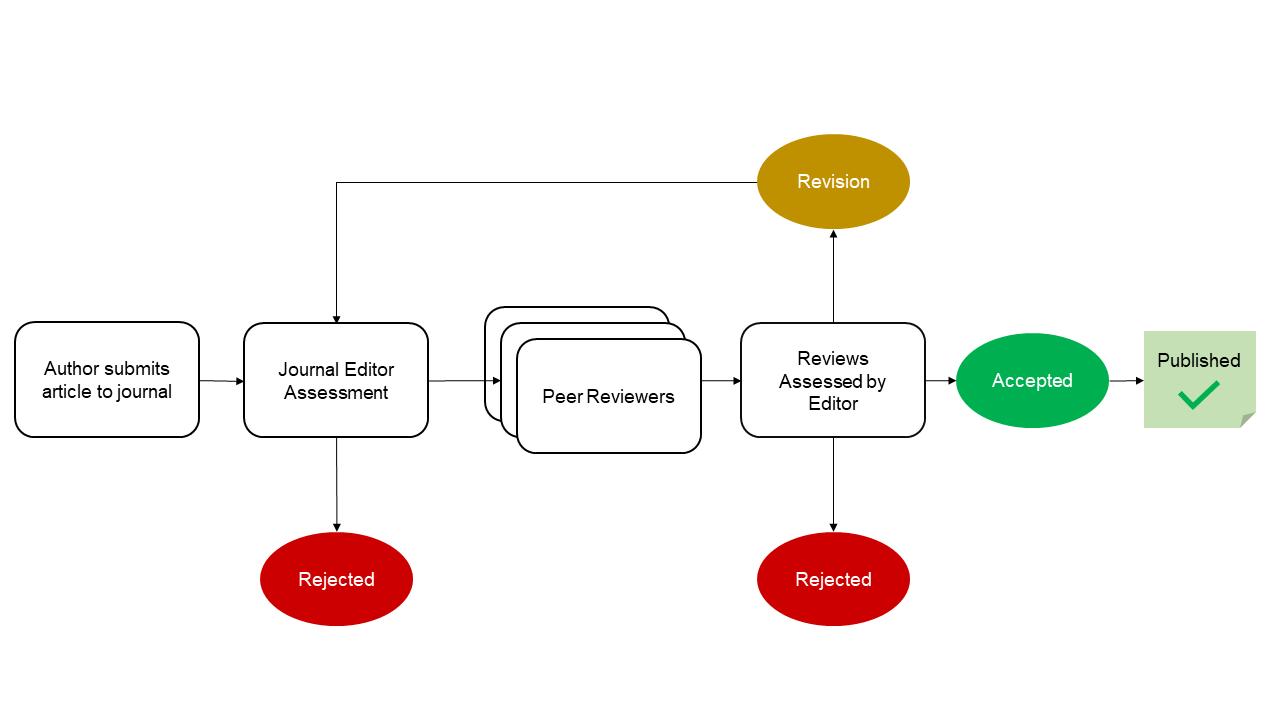
\includegraphics[width=0.8\textwidth]{figures/publishing-process.png}
  \caption{The publishing process} \label{fig:publishing-process}
\end{figure}

Peer reviews can be classified by how identities of parties are managed. In a double-blind review, only the editor knows the identities of the author and the reviewer. In a single-blind review, the name of the reviewer is hidden from the author to let the reviewer criticize without worrying about personal relationships or conflict of interests. The third and emergent form of the peer review is open peer review where the identities of both author and the reviewer are known to each other. In some forms of the open peer review, the identities and the review reports are also publicly available \parencite[4]{HorbachS.P.J.M..2017}, and therefore reviewers can gain credit for their work. Although, the term "open peer review" not only encompasses the openness of identities and the content, but also used for the open participation and transparency of the whole process \parencite{RossHellauer.2017}.

Peer review takes place in many different forms and employs different processes and it’s difficult to acknowledge it as a single system \parencite[2]{HorbachS.P.J.M..2017}. But its essence and rationale are shared among all different applications. Emerged among earlier scientific societies as an internal scrutinization for the scientific quality of manuscripts, it held its importance throughout the proliferation of the printing press, globalization of science after World War II \parencite{Fyfe.2017}, and the adoption of information technologies. It is still perceived by some as the gold standard in scientific publishing \parencite{Mayden.2012} and provides legitimacy for the generated knowledge \parencite{Tennant.2020c}.

\section{Problem Statement} \label{sec:problem-statement}

It is widely accepted that peer review plays an important role in research \parencite{Publons.2018, Taylor&Francis.2015, Ware.2008, Zuckerman.1971}. Despite its importance, peer review is shown to be far from being perfect, by being prone to biases \parencite{Lee.2013, Mahoney.1977}, inconsistencies \parencite{Peters.1982, Rothwell.2000}, and being ineffective in detecting errors \parencite{Schroter.2004}. It usually takes 3 to 5 hours (\cite[146]{Mulligan.2013}; \cite[42]{Ware.2008}) to complete a review and it usually takes more than 3 months for a paper to be accepted \parencite[51]{Ware.2008}. The process is often slow for authors and time consuming for reviewers. Reviewers who are academics themselves with various duties are often not compensated for their review work and they don’t receive credit for their work. Given that number of publications is growing each year \parencite{Bornmann.2015} and each manuscript typically requires 2 to 3 reviewers the peer review system is being put under growing pressure. This situation is said to cause “reviewer fatigue” \parencite{Breuning.2015}. At the same time, editors are reporting that it is getting more difficult to find suitable reviewers, indicated by the increasing decline rates to review invitations \parencite{Baveye.2011, Fox.2017}. 

Despite the numerous deficiencies of the process, it is argued that there is no consensus on an alternative \parencite{Smith.2006, Young.2003} and it is currently the best method ensuring the soundness of scientific publishing (\cite[5201]{Grainger.2007}; \cite[2]{HorbachS.P.J.M..2017}). A range of innovations aimed to tackle the stated problems failed to provide a cure and the peer review remains mostly unchanged \parencite{Tennant.2017}. 


\subsubsection{Peer Review Lacks Incentives}

Some of the problems of peer review are believed to be results of the lack of incentives to review \parencite{Derraik.2015, Willis.2016}, and there’s an ongoing discussion on how to increase researchers’ engagement in reviews in the light of these problems \parencite{Derraik.2015, Gasparyan.2015, Hauser.2007, Squazzoni.2013}. The lack of incentives has its roots within that today the measures and indicators of academic performance are the number of papers published, number of citations, or other citation based scientometrics. These measures play an important role in deciding who climbs up the ranks, who gets hired, or who receives the funding. Despite its importance, peer reviews usually are not recognized as a research output as the manuscripts and do not contribute to researchers’ perceived academic performance \parencite{Tennant.2017}. Therefore, researchers are disincentivized to do reviews and incentivized to publish more manuscripts.

The reliance on publishing-related metrics has also other consequences on peer reviewing. The state of affairs creates the mindset of “publish or perish”: the constant pressure to publish more and get cited more \parencite{Rawat.2014}. Yet, the way to publish more and get cited more is not only doing more research. One can publish the results of their work in smaller and less coherent slices \parencite[4]{Ferreira.2016} in an act called “salami publication” \parencite{SupakSmolcic.2013}. The act is considered unethical \parencite[238]{SupakSmolcic.2013} and with each paper reviewed by multiple reviewers, it puts more pressure on the peer review system \parencite[4]{Ferreira.2016}. This effect is amplified when a paper gets redundantly reviewed in different journals i.e. when authors go “journal shopping”. In this case, following a rejection by a journal with a higher impact, authors continue submitting their papers to gradually lower impact journals until their papers get published while the new editors and reviewers of the submitted paper are not aware of the previous reviews done \parencite[10]{Kovanis.2016}. 

If everyone publishes more and reviews less, then who is doing all the reviews? A strong imbalance in the peer review system was observed where a larger percentage of the peer reviews are done by a minority of researchers and thanks to them there is a sufficient supply of reviewers (\cite{Kovanis.2016}; \cite{Petchey.2014}; \cite[37]{Ware.2008}). Those “peer-review heroes” bear the burden by reviewing much more than they publish \parencite[9]{Kovanis.2016}. The situation raises the concerns that the system may be in a “tragedy of the reviewer commons” \parencite{Hochberg.2009} where participants of the system are encouraged to exploit the system by submitting more papers and less incentivized to do peer reviews. 

There’s a consensus among researchers that an improvement in peer review incentives would enable better reviews \parencite{Publons.2018}. Attracting more reviewers to the reviewer pool would also help balance the heavy burden placed on the reviewing system potentially letting editors find reviewers easier and shorten the time taken from submission until the publication of a manuscript. 

\subsubsection{Closedness of Reviews Prevents Their Acknowledgment}

The practice of blinded reviewing is a feature of the process that hinders public review acknowledgement. Today most of the peer reviews are done as single or double-blind \parencite{Wolfram.2020}. Even though open peer review seems to be gaining popularity \parencite{Wolfram.2020}, scientists are more likely to accept review requests when their identities are hidden \parencite{vanRooyen.1999} and majority of the researchers still prefer blinded reviews over open peer reviews (\cite[149]{Mulligan.2013}; \cite{Taylor&Francis.2015}; \cite[1038-1039]{Wolfram.2020}). It is likely the majority of peer reviews will remain blinded as the anonymity is considered necessary for strong and unbiased scrutiny \parencite[21-23]{RossHellauer.2017}.

However, a problem the closedness of reviews introduces is the difficulty to verify reviews. Since the whole review process takes place internally in journal management systems it is not possible to find out externally if a researcher has really done a peer review for a specific manuscript or a journal, without explicitly contacting the journal. In most of the cases, the transaction costs of contacting a journal is too large for a review, as virtually none of the journals has such a verification system. For reviewers to gain recognition for their work, it is essential that they can easily prove the authenticity of their reviews. The researchers may then showcase their review works done for specific journals and articles publicly or present them when needed as a demonstration of expertise in a field e.g. in job and grant applications. It may also highlight the reviewing workloads of researchers to their employers \parencite[2]{Raoult.2020}. 

Employers are increasingly resorting more to citation-based metrics for assessing their researchers \parencite{Bianchi.2019, Cantor.2015, Kachewar.2013, Verissimo.2013}. These metrics may be taken into account when assessing academic performance \parencite[11]{Ferreira.2016}. Availability of peer review contributions or related metrics may also bring incentives to do more reviews and reduce the imbalance in the review workloads \parencite[4]{Petchey.2014}. 

\subsubsection{Existing Peer Review Showcase Platforms Are Becoming the Sole Owners of Peer Review Data}

There are already running projects that aim to incentivize peer reviews by letting reviewers showcase their work. Since the review data is not publicly available, these "showcase platforms" can track the review contributions of a researcher for them, and verify the reviews they add to their profiles. By providing this verifications service, they act as a trusted third party between the reviewers and  and the bodies potentially interested in this information such as editors, funders, universities or agencies.

Reviewer Credits \footnote{https://www.reviewercredits.com}  is a project to let reviewers certify peer review activity, display their review records, and earn rewards such as books, and discounts to paid publishing services. Reviewers can claim their activity either through automated data transfer between the platform and journal or by Reviewer Credits manually contacting the publisher. \acrshort{ORCID}\footnote{https://orcid.org} also lets users add reviews to their profiles from open review journals or if the journal is an \acrshort{ORCID} member and provides review data to the platform though its \acrshort{API} \footnote{https://info.orcid.org/whats-new-with-peer-review-on-orcid/}. The more popular platform providing a similar service is Publons. Founded by Andrew Preston and Daniel Johnston in New Zealand in 2012 it quickly gained popularity and was welcomed by many academics \parencite[266]{Smith.2015} and was eventually acquired by Clarivate Analytics in 2017. As of November 2020, Publons claims to have over 2 million members\footnote{http://web.archive.org/web/20201109015743/https://publons.com/about/home}. On Publons, researchers can create a profile and add the reviews they have done. To add a peer review, they can either follow a link provided by the journal with a Publons integration after submitting their review or they can manually forward their review acceptance emails to Publons, who then manually verifies the review. By gathering publications and reviews, researchers can showcase their scholarly efforts and earn badges and awards such as “Top Reviewer” or “Highly Cited”. 

These platforms help researchers gain credit for their review contributions, but the proprietary status and of the review showcasing platforms and its potential implications may not be well aligned with the open science goals. Open science is a broad term used for different aspects of science and how science is conducted and there are different definitions of the term. \cite{VicenteSaez.2018} define it as knowledge generation with the four characteristics: transparent, accessible, shared, and collaborative by analyzing the use of term throughout the literature. \cite{Pontika.2015} created a taxonomy by braking down the the broader term "open science" into hierarchical components to provide a consistent terminology and to map the concepts around open science. \cite{Fecher.2013} identify five  schools of thought under the open science discourse, each aims for "opening" different aspects of the knowledge creation process. 

\begin{itemize}
    \item \textbf{Public School:} Open participation of the knowledge creation process, making science comprehensible for common citizens.
    \item \textbf{Democratic School:} Accessibility and transparency for the created knowledge: Open Access, Open Data
    \item \textbf{Pragmatic School:} Improving collaboration, stimulating knowledge dissemination.
    \item \textbf{Infrastructure School:} Providing researchers open tools for dissemination and collaboration 
    \item \textbf{Measurement School:} Finding new ways to measure researchers' impact, recognizing formerly invisible scientific contributions
\end{itemize}

Overall, open science aims to increase the rigour, accountability, and reproducibility in research and "to make research more open to participation, review/refutation, improvement and (re)use for the world to benefit" \parencite{Bezjak.2018}.

\begin{figure}[htpb]
  \centering
  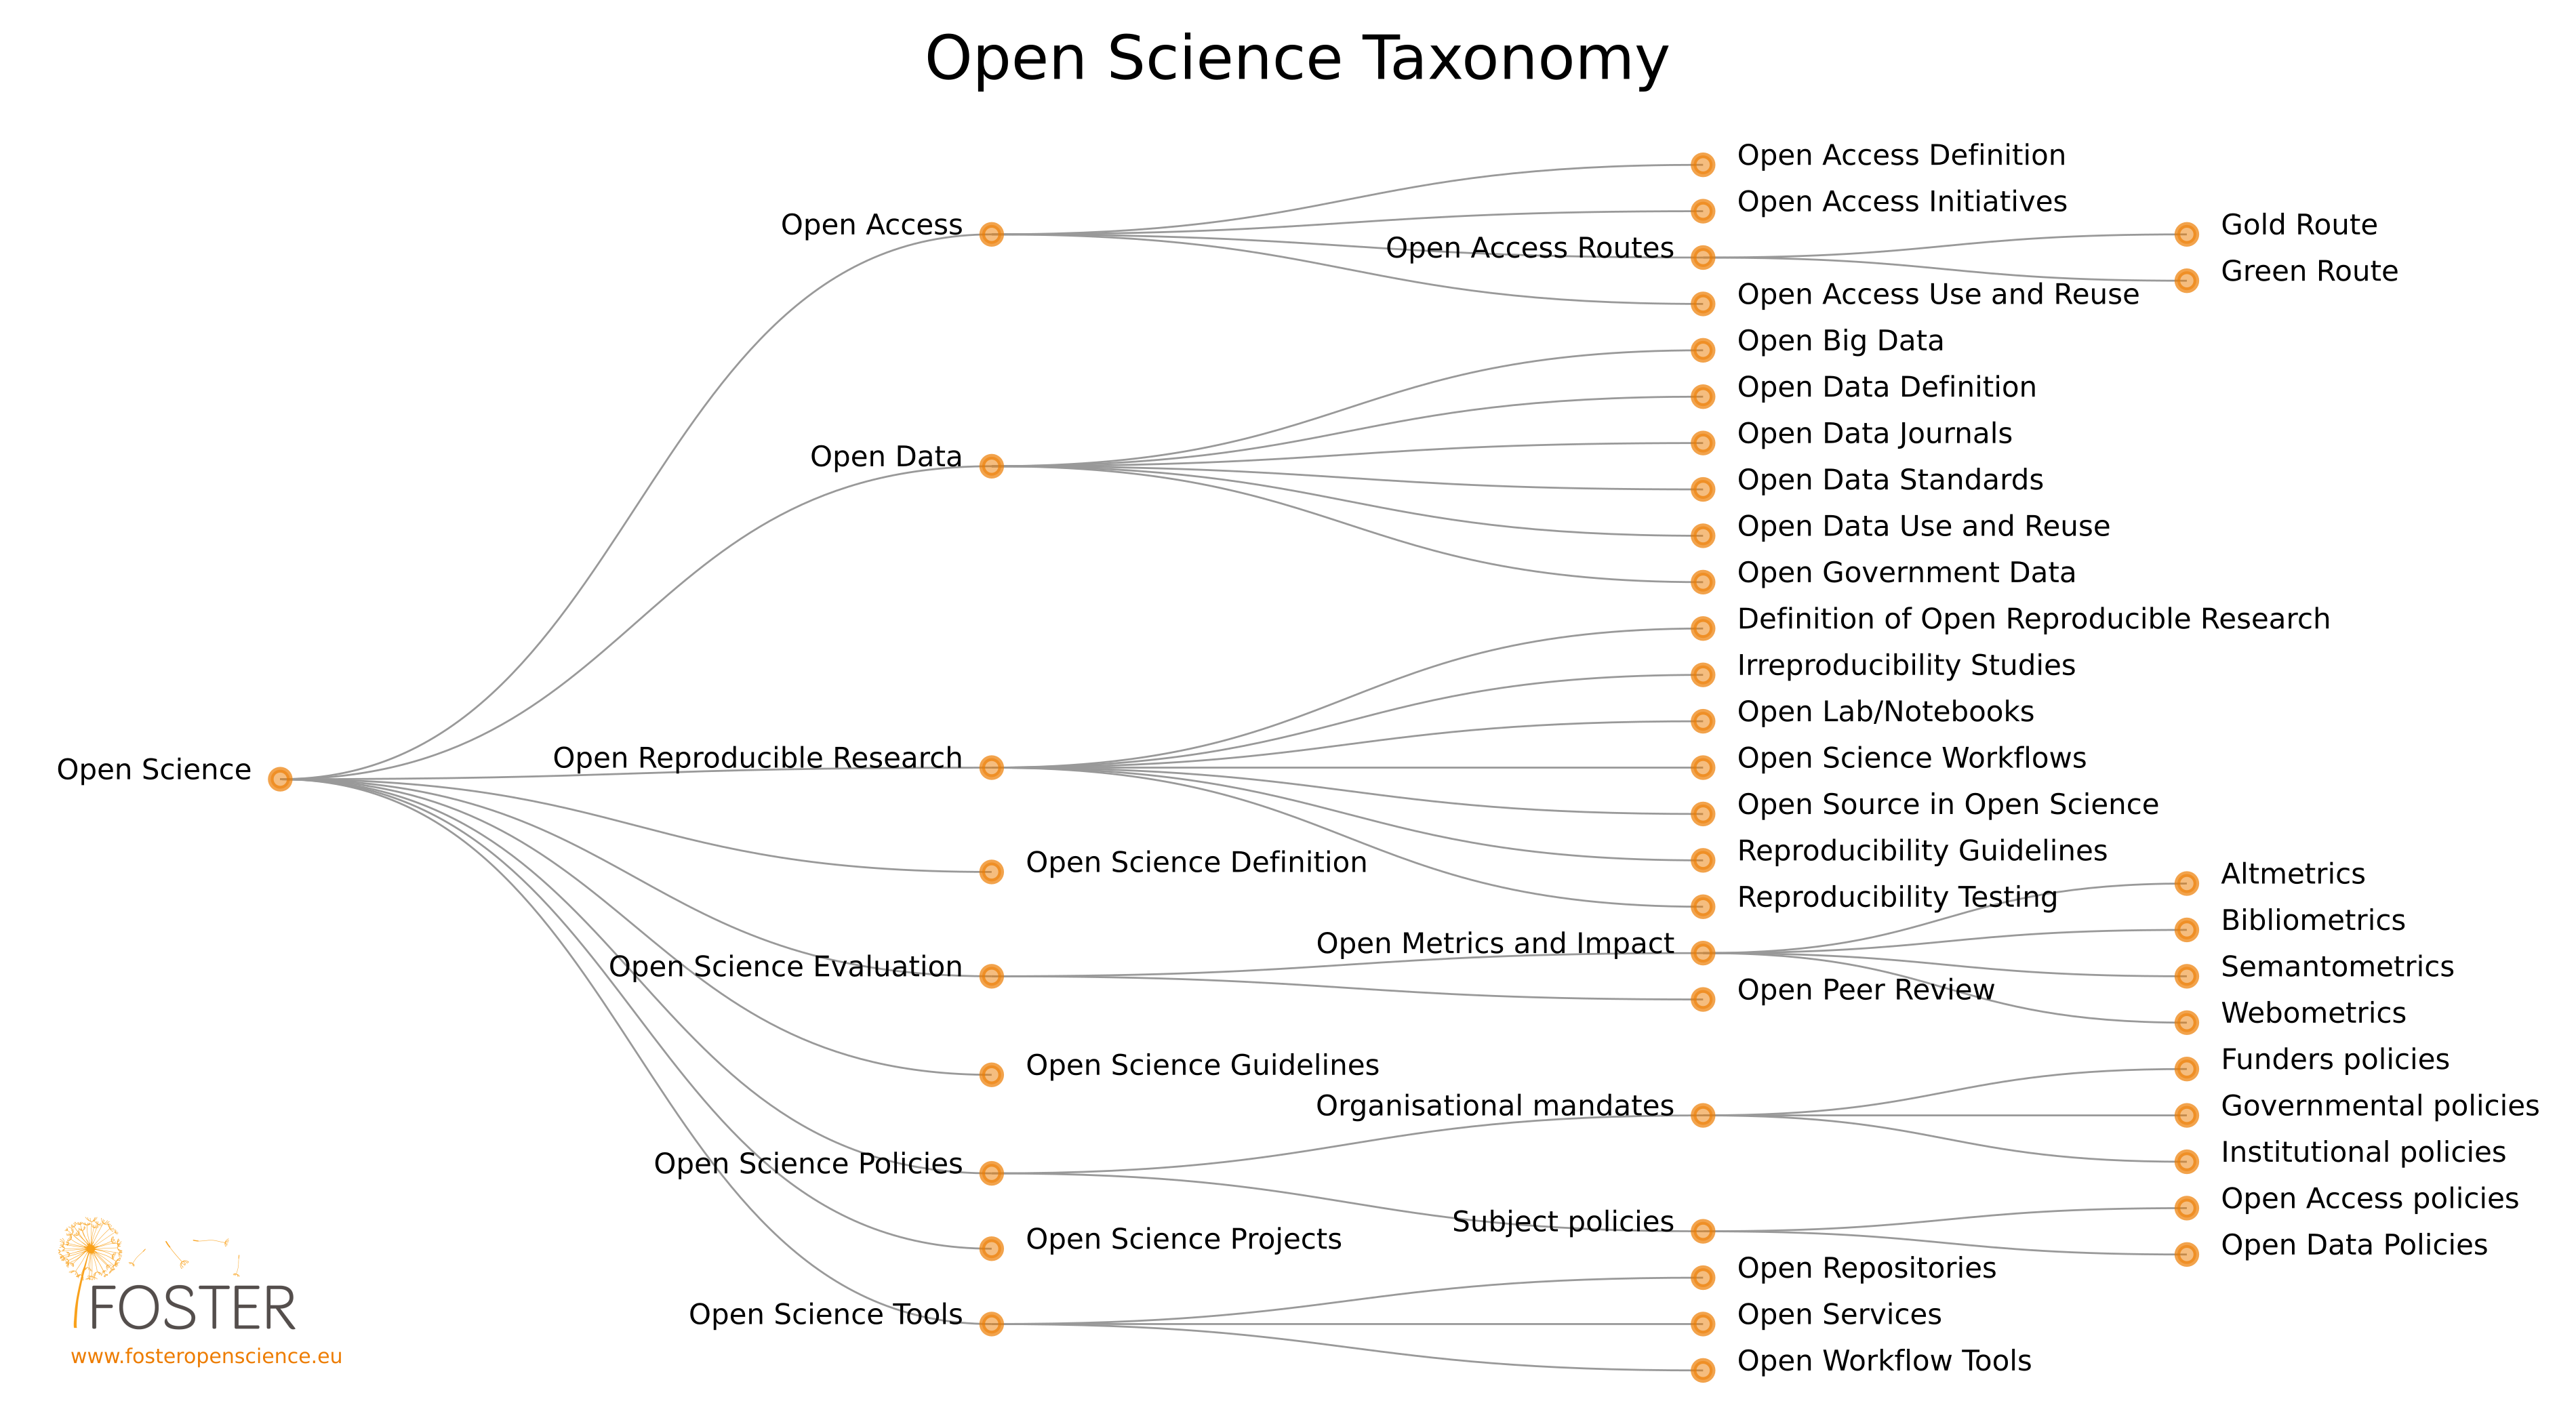
\includegraphics[width=0.8\textwidth]{figures/FOSTER.png}
  \caption{\parencite{Pontika.2015}} \label{fig:foster}
\end{figure}

Despite Publons being accepted by many scientists, it’s pointed out that its metrics may be biased \parencite{Ortega.2019}, and it may be failing to distinguish authentic reviews \parencite{TeixeiradaSilva.2020}. Current verification process by Publons, in particular the verification through review receipt emails, is not transparent. Publons lets users add reviews to their profiles by forwarding the "Thank you for your review" responses of journals. An email response is an easily forgable and unverifiable message. There are no studies on the peer review data if this problem is practically relevant, but there exist fake reviews \footnote{https://retractionwatch.com/2015/08/17/64-more-papers-retracted-for-fake-reviews-this-time-from-springer-journals/} \parencite{Qi.2017, TeixeiradaSilva.2017} and predatory journals wanting to exploit scientific metrics \parencite{xia2015publishes, demir2018predatory}, and credential fraud in science is well known \parencite{Wilson.2020}. Besides, on Publons it is not possible to see how the verification is done and there is no distinction on the platform between an email verification and a verification through a journal integration. Effectively, Publons has to be trusted for the data they provide.

Besides, the fact that the data on the platform is owned by Publons, and effectively Clarivate Analytics, brings the accessibility of the data into question. The platform’s provided API does not provide much data and existing studies making use of the Publons data extract it using web crawlers \parencite[952]{Ortega.2017} which is not allowed without Publons’ written consent according to the platform’s terms\footnote{https://web.archive.org/web/20210414004129/https://publons.com/about/terms/}. The platform appears to have provided data to researchers when requested \parencite[12]{Kovanis.2016}, however there are no guarantees that the data will remain freely accessible as long as it is owned by a proprietary company. Concerns have also been expressed for the transparency of the data previously provided by Clarivate Analytics (\cite{Rossner.2007}; \cite[3]{TeixeiradaSilva.2019}), as the provider of the Journal Impact Factor, and for the fairness of its practices \parencite{TeixeiradaSilva.2013}. A non-profit may be better suited for keeping this data open and accessible. But, currently in the case of \acrshort{ORCID}, which is a non-profit, the journals need to become paid \acrshort{ORCID} members and integrate their \acrshort{API} to be able write the review contributions of the researchers.

The aggregation of peer review data by proprietary parties might also be inappropriate for publishers and journals. The journals are effectively giving away their valuable review data to Publons for free. In turn, Clarivate Analytics processes this data and makes use of it for their profit. An example is the editor matching tool Publons has that lets editors find suitable matches for peer reviews of a manuscript\footnote{https://publons.com/benefits/reviewer-connect}. This itself may not be undesirable, as the fees may be justified by the value it provides for its users. But a single party aggregating the data has a higher risk of causing disagreements with publishers. If a publisher is unwilling to provide review data to a potential competitor, this may hinder the review coverage of the platform. Ideally, a platform should remain an open non-profit, or a joint organization governed by different stakeholders of the whole peer review ecosystem.

The problems of centralization in publishing is apparent \parencite{Lariviere.2015} and there is ever more demand for open science \parencite[1-3]{Piwowar.2018}. As long as the world’s peer review data is under the control of a single party, there exists the possibility for the sole owner of the data to restrict access to it, or start charging fees. This privileged position of the showcasing platforms are due to the role they play as trusted third parties in review verification. If these third parties can be disintermediated, and direct trust can be established between reviewers and consumers of the review data, a review showcasing system with more transparency, open standards, and open data may be possible.

\section{Research Question}

Peer review is a broad and controversial topic with many conflicting perspectives. The process also has many problems outlined that is interconnected with the other aspects of scientific epistemology and the current scientific publishing specifically. It is important to have a narrow focus to be able to analyze the specific problems and to bring impactful solutions. With the problems in peer review identified we focus on the implications of trusted third-parties in peer review verification and recognition and define the following as our research question: \\ 

\begin{center}
    \textit{How can closed peer reviews be verified without trusted third-parties?}
\end{center}

\section{Methodology}

As the work is exploratory and it is goal is to create an improved artifact that will enable the verification of closed peer reviews without a trusted third-party, it is suitable to structure the research process according to a design science framework. For this work the \acrfull{DSRM} proposed by \cite{Peffers.2007} is taken as a guideline for conducting research. The proposed framework presents a nominal process model that can be followed when conducting design science research in information systems. The authors suggest dividing the research process into 6 steps as shown in Figure \ref{fig:dsrm}. The process is not necessarily linear. During the research, the knowledge generated when creating the artifact can be used to refine and improve the artifact, and the improvement of the artifact yields more applicable knowledge. This cycle may be repeated multiple times until the artifact reaches the desired state. Additionally, it is possible to start the research process from the four entry points:

\begin{itemize}
    \item \textbf{Identify Problem \& Motivate:} Problem-Centered Initiation
    \item \textbf{Define Objectives of a Solution:} Objective-Centered Solution
    \item \textbf{Design \& Development:} Design \& Development Centered Initiation
    \item \textbf{Demonstration:} Client/Context Initiated
\end{itemize}

A problem-centered initiation is adopted for our research process. 

\begin{figure}[htpb]
  \centering
  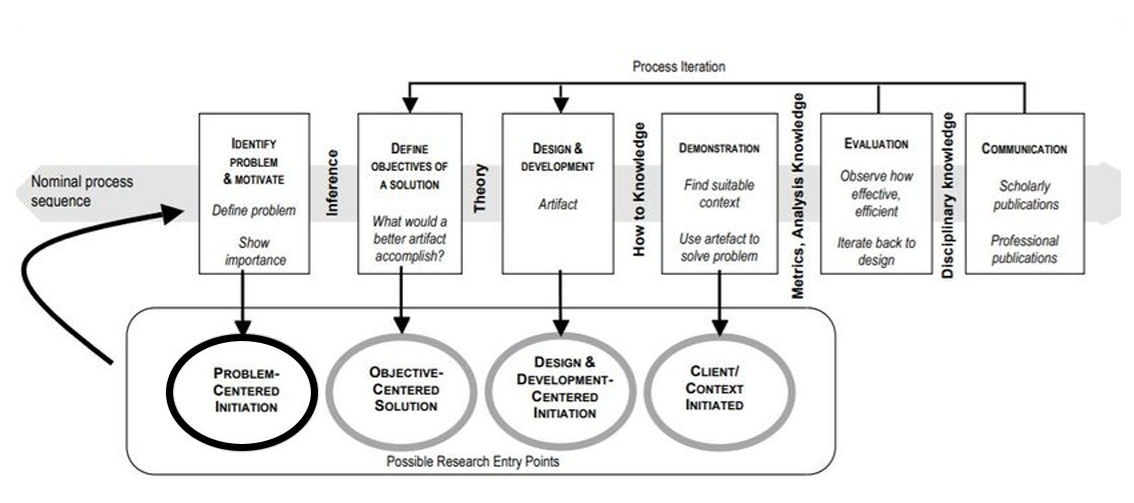
\includegraphics[width=\textwidth]{figures/dsrm.png}
  \caption{Design Science Research Methodology framework proposed by \cite{Peffers.2007}} \label{fig:dsrm}
\end{figure}

\subsubsection{Problem Identification}

We start with the problem identification where we take the \textit{peer review incentive problem}. The problem statement is given in detail in Section \ref{sec:problem-statement} but here we provide how our research brought us to the problems stated. The incentive problem encompasses that researchers are often busy with publication related work and, they are not incentivized to do voluntary peer reviews but instead are incentivized to publish more. This puts a burden on the reviewer resources available and this creates a typical tragedy of commons situation \parencite{hardin2009tragedy, Hochberg.2009} for the reviewer resources available. Further research in the literature uncovers the other problems in peer reviewing such as its quality, the long duration of the review process, and the increasing rejection rates, and that these problems can be traced back to the lack of incentives to do peer reviews. Solution proposals in the literature can be categorized in two groups: the ones that propose monetary incentives for doing peer reviews, and the proposals that focus on bringing recognition to the review contributions of researchers. The latter is also a benefit of open peer review that its proponents often state. This also shows the inherent dilemma of the peer review between keeping the reviews objective and unbiased, and making the process transparent and accountable, which stems from the practice of blinded reviews. Further, it reveals that the lack of recognition to peer reviews is due to the nature of the process, that the identities and contents of peer reviews are hidden and not shared publicly. Our research brings us to the platforms that aim to bring recognition to both open and closed reviews, namely the \textit{peer review showcasing platforms} e.g. Publons. 

Even though these platforms provide value to its users we identify some concerns about Publons. Also from an open science perspective and considering the practices of the centralized large publishers \parencite{Lariviere.2015} we identify problems related to transparency and centralization, and potential practices by the platform undesirable in terms of open data and open access. We pinpoint that these originate from the role these platforms take as \textit{trusted-third party} verifiers, and derive our main goal specifically from this. 

\subsubsection{Defining Objectives}

Considering the outlined problems, we define the main goal of the work as "How can closed peer reviews be verified without a trusted third-party?". Additionally, to design an artifact that achieves the main goal of the work, and to solve other specified problems we define a set of requirements (Section \ref{sec:requirements}) the designed artifact should satisfy. 

\subsubsection{Design and Development}

Based on the requirements we design the artifact using the \acrlong{VC} and \acrlong{zk-proofs} that allows the verification of closed reviews without a trusted third-party. We also describe a showcasing platform that allows the aggregation of reviews and lets researchers build a "peer review resume". We present the technical details of the designed artifact such as the defined peer review vocabulary and the conceived peer review credential. Additionally, we discuss the design decisions, and describe the main user flow in the system. 

\subsubsection{Demonstration}

We develop and deploy a working prototype as a proof-of-concept, and to demonstrate the technical feasibility of the artifact. We give an overview of the architecture of the prototype and demonstrate how users can interact with it. 

\subsubsection{Evaluation}

We evaluate the work qualitatively through interviews with academics that are familiar with the peer review process and the peer review showcasing platforms.

%% TODO: TAM framework

\subsubsection{Communication}

Finally, the work is communicated in the form of a thesis document, and the open source code is shared on \href{https://github.com/kuzdogan/peer-review-verifiable-credentials-thesis}{GitHub} with instructions how to use the deployed prototype. 


\section{Related Work}

The problems in peer review caught the attention of scientists. Besides the descriptive literature on peer review’s shortcomings, a variety of works discussed and prescribed solutions to the incentive problem. An often encountered suggestion is to ask researchers to do sufficient reviews to balance the system, usually 3 reviews per paper, a “quid pro quo” (\cite{Derraik.2015}, \cite[5201]{Grainger.2007}). To maintain the timeliness of the process \cite{Hauser.2007} suggest a punishment for reviewers who return their reviews late and a reward for the ones returning on time. \cite{Ferreira.2016} suggest making peer review mandatory and paying the reviewers and calls for a decoupling of the peer review system from the scientific publishing by founding a Global Peer Review Platform. Direct monetary compensation of reviewers was also suggested many times \parencite{Prufer.2010}. \cite{Fox.2010} suggest a credit system where authors have to pay for their submissions and earn by conducting reviews, effectively “privatizing the reviewer commons”. Others proposed crypto-economic models through peer review tokens on a blockchain that will work as credits for peer reviews or as reputation indicators \parencite{Avital.2018, Jan.2018c, Spearpoint.2017, Tarkhanov.2020}. Also using a blockchain-based token and lotteries \cite{Janowicz.2018} provide a model for how integrating distributed ledger technologies could benefit the Semantic Web journal’s processes. \cite{TenorioFornes.2019} suggest a whole publishing system that is decentralized using Ethereum and IPFS. Ants-Review suggests an Ethereum based incentive system with its native token ANTS that allows bounties for open anonymous peer reviews \parencite{TrovoMassari}.

\section{Structure}

The rest of this work is structured as follows: \hyperref[chapter:background]{Chapter 2 (Background)} introduces the technical foundations in this work that are required for the creation of and to understand the proposed solution. \hyperref[chapter:design]{Chapter 3 (Design \& Implementation)} outlines the requirements defined for the designed artefact and describes the design of the proposed system. Here the details of the artefact are laid out and the design decisions are communicated. Next in this chapter, the implemented prototype is described, which demonstrates the technical feasibility of the conceived design. A comparison between the conceptual design and the implemented prototype is also provided. \hyperref[chapter:evaluation]{Chapter 4 (Evaluation)} involves the evaluation of the designed artefact based on the interviews with researchers. \hyperref[chapter:discussion]{Chapter 5 (Discussion)} shares the learnings gained in the process, and discusses potential future work and considerations. Finally, \hyperref[chapter:conclusion]{Chapter 6 (Conclusion)} presents the conclusions.